% Drawing 79/15-9 -- folder 79, batch 15, archive page 286 (PDF page 287).
% Transcription: un hexagone dont tous les sommets sont joints entre eux.
% Kind: hexagon with all diagonals (K6). Method 3 (encoded, rendered from the data). Status: ok.
% Notes: Hexagon with all its vertices joined: the complete graph K6. Encoded as a graph (polyhedron/1 with extra_edges): V 6, E 15. Vertex names 1..6 are ours.
% Coordinates: 1 unit = 1 mm = 1/100 of the crop width (bbox in page fractions: [0.58, 0.1, 0.8, 0.25]).
% Redrawn by Claude (claude-opus-5-5), issue #73, 2026-11-07; not checked by a human; not compiled (no TeX in the session).
% Rights: reproduces part of the work -- behind RENDER_TRANSCRIPTS, never published by itself.
\documentclass[tikz,border=3pt]{standalone}
\usepackage{amsmath,amssymb}
\usetikzlibrary{patterns,arrows.meta}
\tikzset{pencil/.style={black!45}, struck/.style={black!35}, mark/.style={circle,draw,inner sep=1.3pt}, pt/.style={circle,fill,inner sep=0.9pt}, opt/.style={circle,draw,fill=white,inner sep=1.1pt}}
\begin{document}
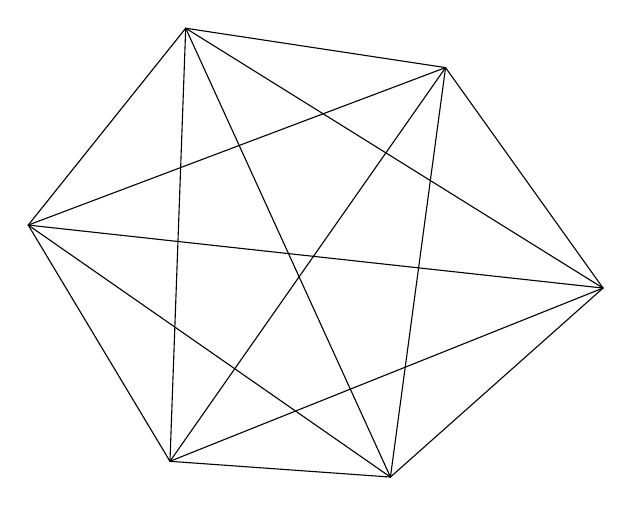
\begin{tikzpicture}[x=1mm,y=1mm,line cap=round,line join=round,font=\scriptsize]
\draw (24,-50) -- (44,-25);
\draw (24,-50) -- (77,-30);
\draw (24,-50) -- (97,-58);
\draw (24,-50) -- (70,-82);
\draw (24,-50) -- (42,-80);
\draw (44,-25) -- (77,-30);
\draw (44,-25) -- (97,-58);
\draw (44,-25) -- (70,-82);
\draw (44,-25) -- (42,-80);
\draw (77,-30) -- (97,-58);
\draw (77,-30) -- (70,-82);
\draw (77,-30) -- (42,-80);
\draw (97,-58) -- (70,-82);
\draw (97,-58) -- (42,-80);
\draw (70,-82) -- (42,-80);
\end{tikzpicture}
\end{document}
